\documentclass[a4paper,11pt]{article}
\usepackage[margin=22mm]{geometry}
\usepackage{fontspec,amsmath,booktabs,graphicx,hyperref}
\setmainfont{STIXGeneral}
\setlength{\emergencystretch}{2em}
\begin{document}
\begin{center}{\Large Affine constructions: complete manuscript costs}\\[4pt]
Human Compression project\end{center}
The source is Hou, Feng and Leemans, \emph{Regular 3-polytopes of order
$2^n p$}, arXiv:2001.02945v2, dated 14 July 2024. We compare its complete
seventeen pages with our complete seven-page common paper and nine-page
application. The exact admitted principal contract has thirty-three rows;
this measurement changes none of its mathematical conclusions.

\paragraph{The combined written comparison.}
Using calibrated NFC characters without whitespace, the costs are
\begin{center}\begin{tabular}{lr}\toprule
Complete document & Characters\\\midrule
Source L012 & 32\,767\\
Common theory $U_{\mathrm{Affine}}$ & 19\,070\\
Application AF1 & 22\,638\\
Whole program appendix & 17\,250\\\bottomrule
\end{tabular}\end{center}
The combined written ratio is
\[
 R_{\mathrm{written}}=\frac{32\,767}{19\,070+22\,638}
 =\frac{32\,767}{41\,708}=0.785629.
\]
Thus the complete written replacement is longer than the source by this
measure. The common paper is charged in full in this topic, including
arguments also available in another topic. It is not discounted because
they were previously proved or counted elsewhere.

\paragraph{The result after acquiring the common material.}
Once the whole common paper and all six complete required programs are
available, the source/application ratio is
\[
 R_{\mathrm{conditional}}=\frac{32\,767}{22\,638}=1.447434.
\]
This is a shorter local application. It does not make the common paper
free in the combined comparison. Titles, context, references, complete
proofs and all local hypotheses remain in every measured document.

\begin{center}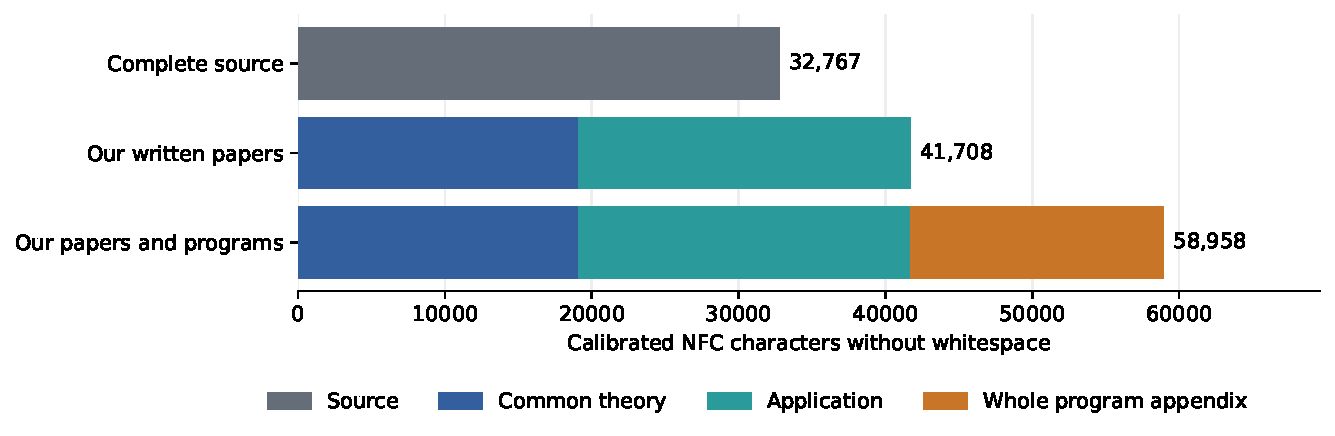
\includegraphics[width=\linewidth]{costs.pdf}\end{center}
\newpage
\paragraph{The complete program boundary.}
The eight-page appendix prints six whole mathematical programs, including
their embedded diagnostics. It is required material in the accepted
scientific edition. Adding it once gives
\[
 R_{\mathrm{programs}}=\frac{32\,767}{41\,708+17\,250}
 =\frac{32\,767}{58\,958}=0.555769.
\]
The six complete raw files cost 16\,682 characters. Substituting this
representation for the printed appendix gives
\[
 R_{\mathrm{raw}}=\frac{32\,767}{58\,390}=0.561175.
\]
The two program representations are alternatives. They are never both
added to the denominator, and no diagnostic fragment is pruned.

Three auxiliary scripts are inventoried separately: the replay driver,
the checks for changed input files and the finite hypothesis diagnostics.
They cost 16\,581 characters in the same NFC coordinate. The original
scientific metadata lists two different pairs; the inventory records
their union of all three files without changing the scientific edition.
The three supporting Lean files cost 7\,958 characters and are separately
recorded as formal validation. These costs are not silently added to a
mathematical manuscript or to the program appendix.

\paragraph{What is included and what remains unknown.}
The numerator is the whole source manuscript for the admitted principal
contract. It does not assert recovery of every auxiliary assertion.
General Problem 1.1, the separate full Table 1 census and the ancillary
uniqueness claim for the two order-384 seeds remain outside that contract.
The source sign correction and all retained external theorems keep their
existing attribution and qualifications. This measurement adds no credit for another source or a solved question.

The independent input review counted all forty-one physical PDF pages.
Only page numbers and repeated running headers are removed. It checked
114 glyph substitutions against the actual encoded bytes and embedded
fonts, and inspected every proposed furniture exclusion. Printed hyphens,
formula ordering and extraction spacing are preserved. The same complete
costs are supplied for three extraction policies, NFC and NFKC, and five
length units: thirty coordinates in all. The CSV tables contain ninety
combined fractions and thirty conditional fractions.

The source's 163 inline graphic marks have an unknown graphic and layout
cost. Its original program files are unavailable. Expanded external
proofs, the SmallGroups catalogue and the construction of exact group
algorithms also have unknown acquisition costs. None is assigned zero.
Consequently these are declared text and program comparisons, not a
measure of all visible mathematical information or research effort.

Nine existing Lean declarations verify specified quotient, period and
sign statements. They do not formalize the entire source contract.
Paired proof dependencies and exclusive passage costs are still pending.
The numerical packet awaits independent arithmetic and reader review;
its input boundary has already been independently accepted.
\end{document}
